\documentclass{article}
\usepackage{amsmath}
\usepackage{amsthm}
\usepackage{amsfonts}
\usepackage{amssymb}
\usepackage{bbold}
\usepackage{dsfont}
\usepackage{graphicx}
\usepackage{cleveref}
\usepackage{bm}
\usepackage{booktabs}
\usepackage{siunitx}
\usepackage{xcolor}
\usepackage[utf8]{inputenc}
\usepackage[english]{babel}
\newtheorem{definition}{Definition}
\newtheorem{example}{Example}
\newcommand{\exP}[1]{\mathrm{e}^{#1}}
\newcommand{\dif}{\mathrm{d}}
\renewcommand{\vec}[1]{\mathbf{#1}}
\newcommand{\pdagger}{{\phantom{\dagger}}}
\newcommand{\state}[1]{\vert #1\rangle}
\newcommand{\cstate}[1]{\langle #1\vert}
\newcommand{\tr}[1]{\mathrm{tr}\left\{#1\right\}}
\newcommand{\trs}[2]{\, \mathrm{tr}_{#1}\{#2\}}
\newcommand{\expc}[3]{\langle #1\vert #2 \vert #3\rangle}
\usepackage[doi=false,url=false,isbn=false,backend=bibtex,style=nature,natbib=true,sorting=none]{biblatex}
\bibliography{bib.bib}
\usepackage{geometry}
\geometry{
	a4paper,
	total={170mm,257mm},
	left=20mm,
	top=20mm,
}
\begin{document}
\title{Report 14: CISS effect within the Ehrenfest method}
\author{Rudolf Smorka}
\maketitle

\section{Dynamics}
Show for $L=1x3$ and $L=2x4$ the dependence on voltage for couple of voltages. 
Show here averaged and single-trajectory runs.
Show dependence on system size for a couple of voltages. 
Insight: Transient charge current dynamics consists of multiple time-scales. The last one, in which the current drops down does not depend on system size and not on voltage. It is determined by electron-vibrational coupling.
Show Magnetocurrent: For $L=1x3$ its strictly zero and $L=2x2$ is the smallest system size to see an effect on the single-trajectory level. 
\section{Steady state}
For obtaining the steady state magnetoresistance $M_R$, the steady state currents $I_P$ under varying lead spin polarization $P$ have to be obtained. As shown in the previous section, there are multiple time scales in the transient dynamics. 
In the last time scale, the charge current does not change significantly with time, apart from oscillations around a time-averaged value. These oscillations arise due to the finite number of trajectories, and their amplitude decreases with increasing number of trajectories. The steady state currents $I_P$ are obtained by averaging the time-dependent, ensemble-averaged current $\langle I_P(t)\rangle$ over the last time scale.
The ensemble averaged current and the time interval for the time average is shown in \cref{fig:Current_dynamics_averaging}. The full lines show $\langle I_P(t)\rangle$ for $P=0.5$, obtained from an ensemble average over 1800 trajectories (72 averages over 25 trajectories each). The shaded area indicates the standard error $\frac{\sigma}{\sqrt{N}}$ obtained from the standard deviation $\sigma$ of the ensemble average, treating the average over 25 trajectories as a single data point (sample size is thus $N=72$). The differently colored lines in the interval $\mathcal{I}=[30,85]\SI{}{\pico\second}$ shows the ensemble averaged current used for obtaining the steady state currents.
\begin{figure}[!h]
	\centering
	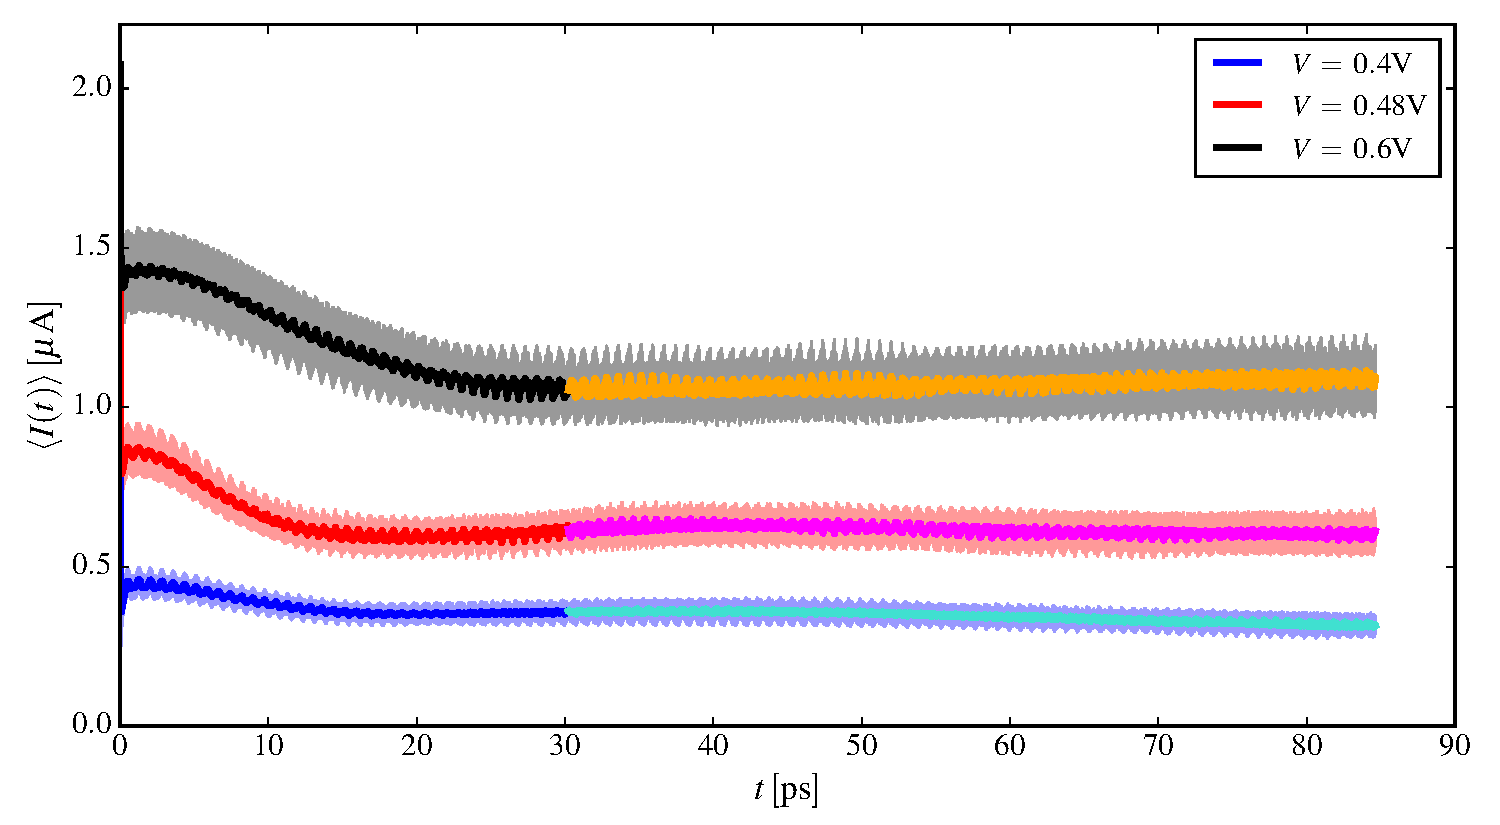
\includegraphics[width=1.0\textwidth]{figs/L2x3_P0.5_VVar_current.pdf}
	\caption{Ensemble averaged charge current for $L=2\times 3$ (full lines) with standard error from ensemble average (shaded area) and the interval used for time averaging (different color on top of ensemble average). The number of trajectories are $n_\mathrm{traj}=1800$ for all shown voltages.}\label{fig:Current_dynamics_averaging}
\end{figure}
The standard deviation $\sigma_{I_P}$ of the steady state current consists of the standard deviation $\sigma_{\langle I_P(t)\rangle}$ on the ensemble averaged current at all times $t\in\mathcal{I}$ 
\begin{equation*}
	\sigma_{I_P} = \frac{1}{N_t}\sqrt{\sum_{t\in \mathcal{I}}\left(\sigma_{\langle I_P^L(t)\rangle}^2+\sigma_{\langle I_P^R(t)\rangle}^2\right)}
\end{equation*}
with the standard deviations $\sigma_{\langle I^{L,R}_P(t)\rangle}$ obtained from the usual definition of the standard deviation. 
\Cref{fig:Currents_SteadyState} shows the steady state current $I_{P=0.5}$ as defined above for various system size and voltage. The errorbars indicate the standard deviation $\sigma_{I_{P=0.5}}$. Here, the standard error is not shown because it is not visible on the shown scale as the number of time points used in the average is $N_t = 5\cdot 10^4$.
In this plot, the black, red and blue data points show the steady state current for voltages $V=\SI{0.4}{\volt},\SI{0.48}{\volt}$ and $\SI{0.6}{\volt}$, respectively, obtained with the new version of the code. The orange dots show the steady state currents for $V=\SI{0.348}{\volt}$ and the orange diamonds the currents for the noninteracting problem. 
Comparing the orange dots with the black dots, the difference is due to different voltages computes. Apart from this difference, the new and the old code agree on the trend of decreasing currents with increasing system size. While currents increase with increasing voltage in the regime investigated here (partial resonance), the relative change of the current with system size seems to be independent of the voltage. This can be seen for example for $\frac{I(L=3)}{I(L=10)}$ which is $\approx 1.8$ for $V=\SI{50}{\volt}$, $\approx 1.9$ for $V=\SI{60}{\volt}$, and $\approx 1.6$ for $V=\SI{75}{\volt}$. 
As a comparison, in the noninteracting problem the current does not change with system size (orange diamonds). 
\begin{figure}[!h]
	\centering
	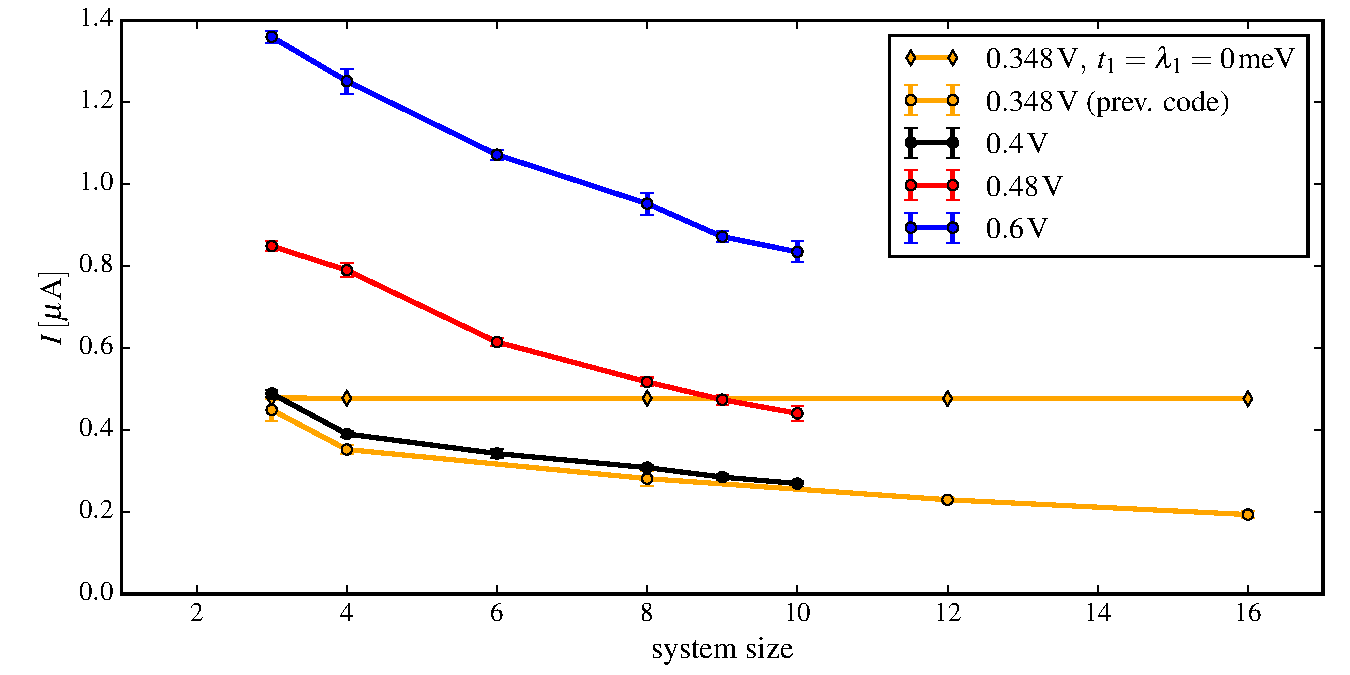
\includegraphics[width=1.0\textwidth]{figs/Currents_sizeVar_P0.5_VVar.pdf}
	\caption{Steady state currents for various voltage (differently colored points) and various system size.}\label{fig:Currents_SteadyState}
\end{figure}
To get a better understanding of the system size dependence of the steady state charge current, \cref{fig:Currents_SteadyState_sqrtN} shows the current scaled with the square root of the system size. For comparison is also shown the scaled steady state current for a non interacting problem with scaled system-lead coupling $\Gamma'=\Gamma_0/\sqrt{N}$. For all investigated voltages, the scaled current for the original problem with electron-vibrational coupling and SOC assisted coupling stays approximately constant with the system size.
Since the scaled currents for a scaled $\Gamma$ also shows a constant dependence on system size, the effect of the electron-vibrational coupling is recovered by rescaling the system-lead coupling.
Also note that the system size dependence shown here is qualitatively in agreement with Franssons results shown in Fig. 2 in \cite{fransson2020vibrational}.  
\begin{figure}[!h]
	\centering
	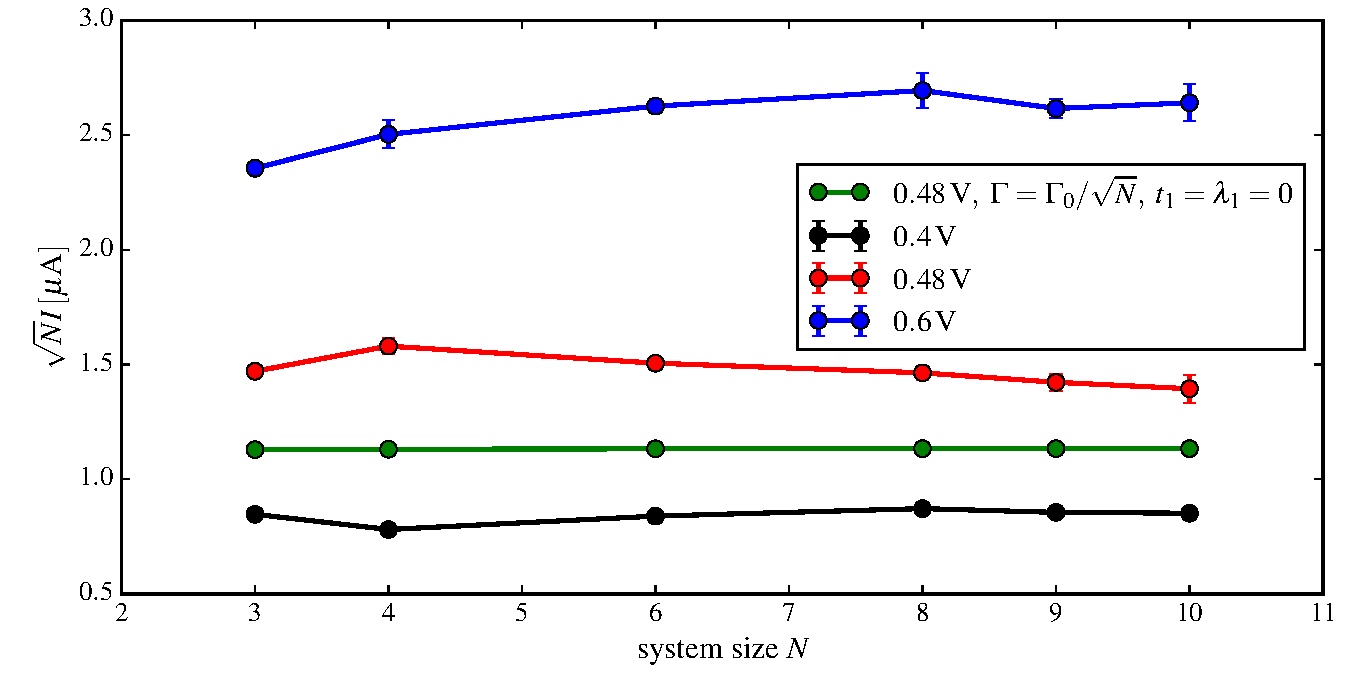
\includegraphics[width=1.0\textwidth]{figs/Currents_sizeVar_P0.5_VVar_sqrtN.pdf}
	\caption{Steady state currents scaled by $\sqrt{N}$ with the system size $N$.}\label{fig:Currents_SteadyState_sqrtN}
\end{figure}
\begin{figure}[!h]
	\centering
	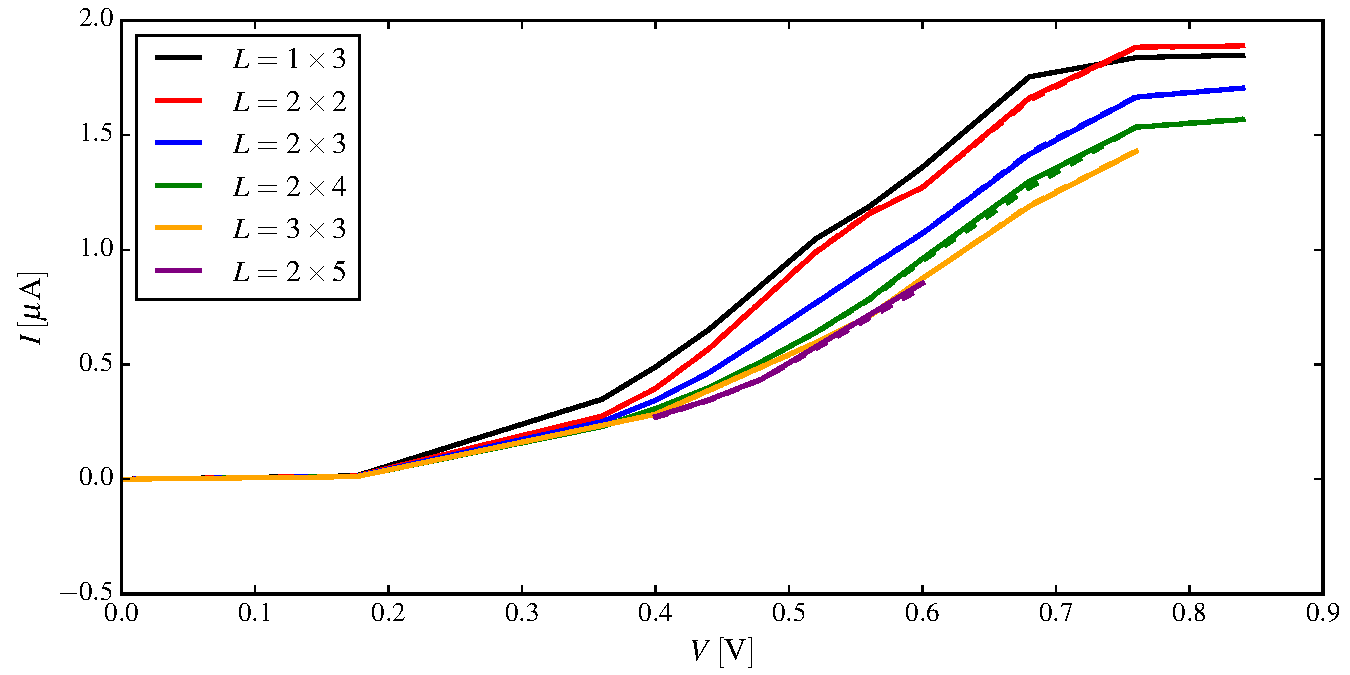
\includegraphics[width=1\textwidth]{figs/IV_sizeVar_PVar_VVar.pdf}
	\caption{Current voltage characteristics for various system size. Full lines are steady state currents for $P=0.5$ and dashed lines for $P=-0.5$.}
\end{figure}
\Cref{fig:Magnetocurrent_std,fig:Magnetocurrent_stderr} show the system size and voltage dependence of the magnetoresistance $M_R$
\begin{equation*}
	M_R=100\left\vert\frac{I_\uparrow-I_\downarrow}{I_\uparrow+I_\downarrow}\right\vert,
\end{equation*}
in which we show the standard deviation $\sigma_{M_R}$ obtained from the standard deviations of the respective left and right currents for $P=0.5$ and $P=-0.5$  in \cref{fig:Magnetocurrent_std}. \Cref{fig:Magnetocurrent_stderr} shows the magnetoresistance with errorbars indicating the standard deviation obtained using the standard errors of the respective currents. The reason for showing both is the same as mentioned above, that is that by time averaging currents, the standard error is very small, even when sample to sample variations are non negligible. While plotting the standard error suggests that the magnetoresistance is a robust quantity, when plotting errorbars obtained from the standard deviation alone it is clear that oscillations of the current due to a finite sample size are not negligible. In particular, the standard deviation captures the strong temporal oscillation of the magnetoresistance, such that, on average, the magnetocurrent is essentially zero (within one standard deviation).  
\begin{figure}[!h]
	\centering
	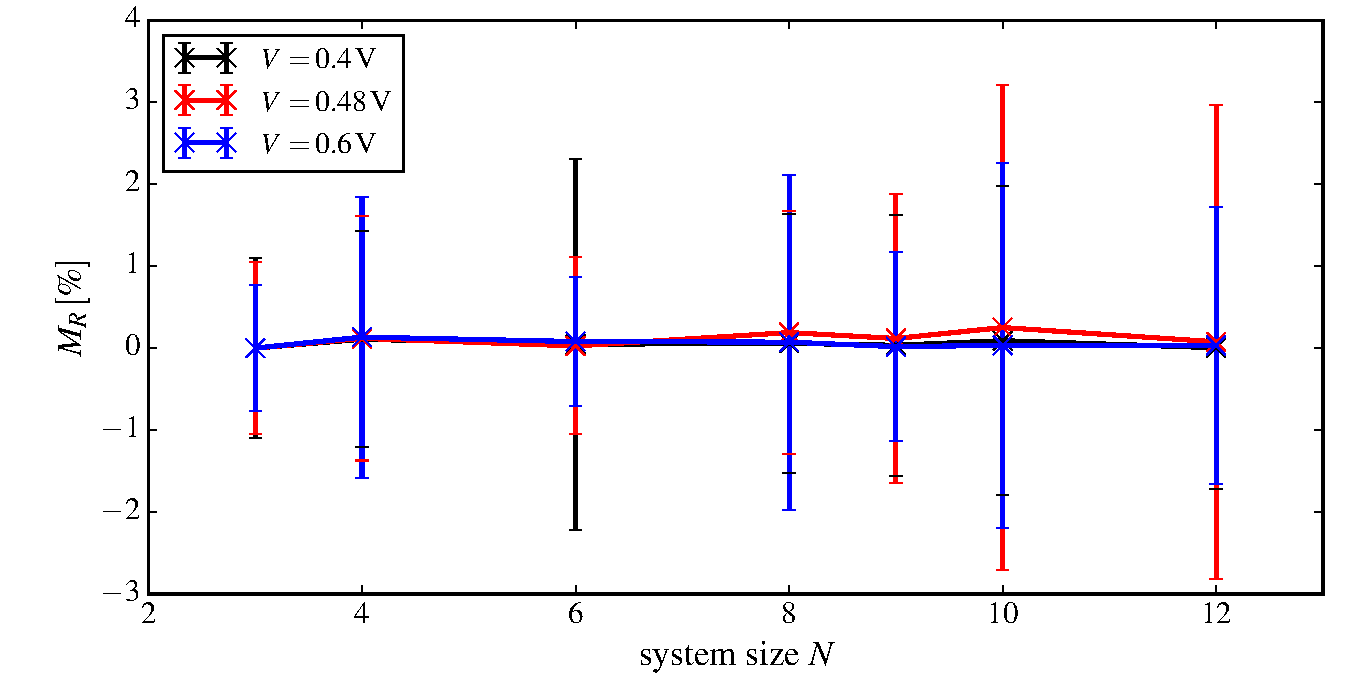
\includegraphics[width=1\textwidth]{figs/Magnetocurrents_sizeVar_VVar_std.pdf}
	\caption{Magnetocurrent: System size and voltage dependence. Error bars indicate error obtained from standard error of the time average of the charge currents.}\label{fig:Magnetocurrent_std}
\end{figure}
\begin{figure}[!h]
	\centering
	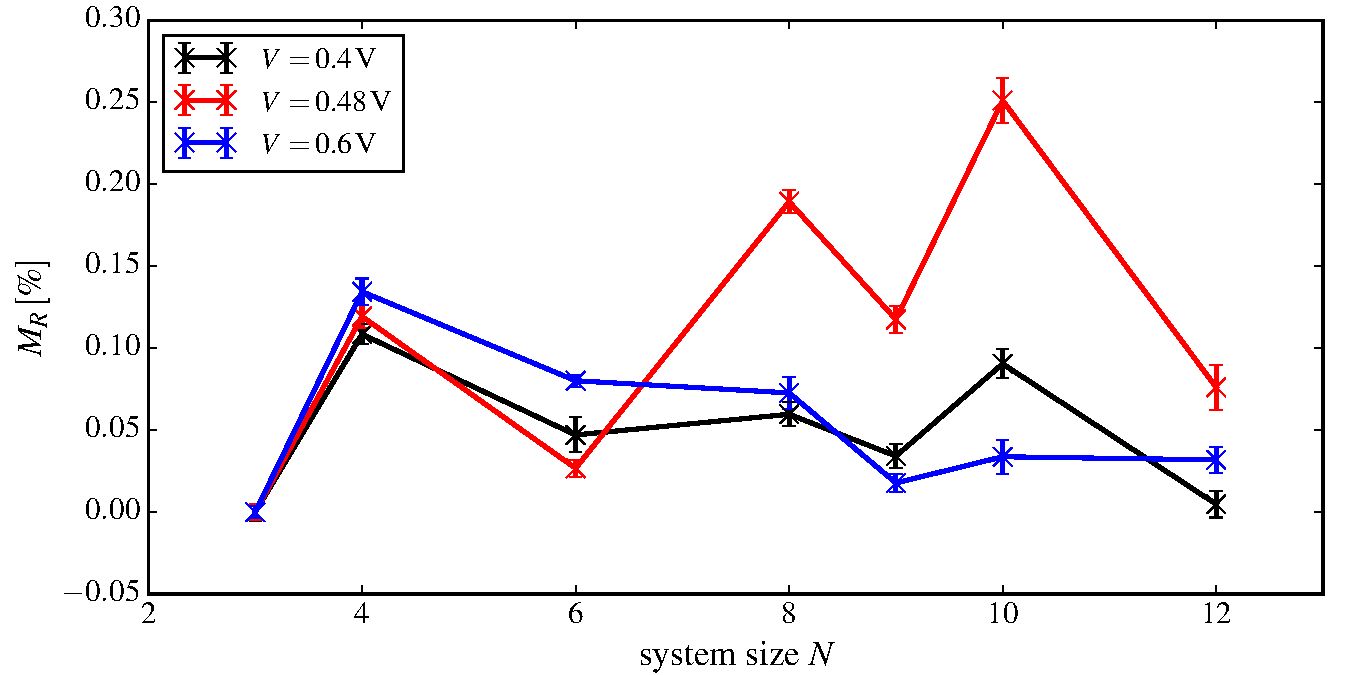
\includegraphics[width=1\textwidth]{figs/Magnetocurrents_sizeVar_VVar_stderr.pdf}
	\caption{Magnetocurrent: System size and voltage dependence. Error bars indicate error obtained from standard deviation of the time average of the charge currents.}\label{fig:Magnetocurrent_stderr}
\end{figure}
Concerning the magnetoresistance, the results shown here are not in agreement with the ones shown in Fig. 2 in \cite{fransson2020vibrational}. For example, for a system size of $L=2\times 4$, Fransson obtains a magnetoresistance of around $5\%$ for $V=\SI{0.6}{\volt}$, while we obtain below $0.1\%$.
\begin{itemize}
	\item Current-voltage for static phonons: $X_i=\langle X(t)\rangle_\mathrm{stat}$ (obtained from full calculation): Is the current drop with system size a purely electronic effect due to rearranged geometry?
	\item Current-voltage for statically disordered phonons: Sample $X_i$ from Wigner, but do not make any propagation of them. Is the static disorder leading to changes in eigenstates (e.g. their localization), which leads to a decrease of the current?
	\item How to obtain memory kernel from the calculations? Compute the position autocorrelation function for phonons.
	\item How to extend the model to three dimensional phonons: Include vibrational mode in $x-y$ plane (inclusion of chirality of phonons), relation to molecular ratchets 
\end{itemize}
\printbibliography
\end{document}

